\section{State Minimization}

The process of reducing a given DFA to its minimal form is called as minimization of DFA.
\begin{itemize}
  \item It contains the minimum number of states.
  \item The DFA in its minimal form is called as a Minimal DFA.
\end{itemize}

The two popular methods for minimizing a DFA are
\begin{itemize}
  \item Equivalence Theorem
  \item Myhill Nerode Theorem
\end{itemize}

\newpage
\subsection{Equivalence Theorem}

\begin{multicols}{2}
\setlength{\columnsep}{1.5cm}
\setlength{\columnseprule}{0.2pt}

\subsubsection*{Step-1}

Eliminate all the dead states and inaccessible states from the given DFA (if any).

\begin{itemize}
  \item \textbf{Dead State:} All those non-final states which transit to itself for all input symbols in $\Sigma$ are called as dead states.
  \item \textbf{Inaccessible State:} All those states which can never be reached from the initial state are called as inaccessible states.
\end{itemize}

\subsubsection*{Step-2}

Draw a state transition table for the given DFA. Transition table shows the transition of all states on all input symbols in $\Sigma$.

\subsubsection*{Step-3}

Now, start applying equivalence theorem.
\begin{itemize}
  \item Take a counter variable $k$ and initialize it with value 0.
  \item Divide $Q$ (\textit{set of states}) into two sets such that one set contains all the non-final states and other set contains all the final states.
  \item This partition is called $P_0$.
\end{itemize}

\subsubsection*{Step-4}

\begin{itemize}
  \item Increment $k$ by $1$.
  \item Find $P_k$ by partitioning the different sets of $P_{k - 1}$.
  \item In each set of $P_{k - 1}$, consider all the possible pair of states within each set and if the two states are distinguishable, partition the set into different sets in $P_k$.
\end{itemize}

Two states $q_1$ and $q_2$ are distinguishable in partition $P_k$ for any input symbol `$a$', if $\delta(q_1, a)$ and $\delta(q_2, a)$ are in different sets in partition $P_{k-1}$.

\subsubsection*{Step-5}

Repeat \textit{step-4} until no change in partition occurs. In other words, when you find $P_k = P_{k - 1}$, stop.

\subsubsection*{Step-6}

All those states which belong to the same set are equivalent. The equivalent states are merged to form a single state in the minimal DFA.

\begin{center}
  \textit{\# of states in Minimal DFA = \# of sets in $P_k$  }
\end{center}

\end{multicols}

\begin{examplebreak}{}
  Minimize the following DFA:
  \begin{center}
    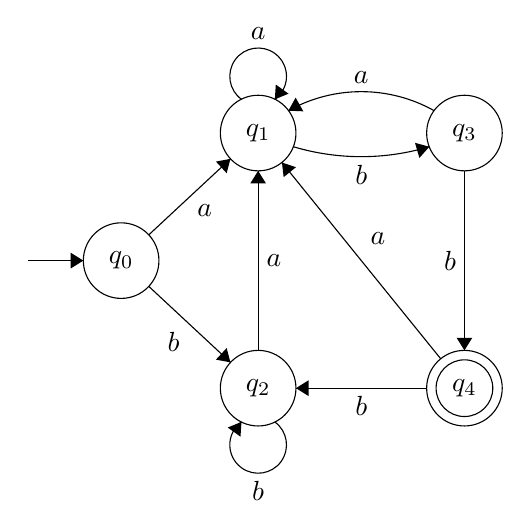
\begin{tikzpicture}[scale=0.2]
    \tikzstyle{every node}+=[inner sep=0pt]
    \draw [black] (6.1,-15.4) circle (2.4);
    \draw (6.1,-15.4) node {$q_0$};
    \draw [black] (14.8,-7.3) circle (2.4);
    \draw (14.8,-7.3) node {$q_1$};
    \draw [black] (14.8,-23.5) circle (2.4);
    \draw (14.8,-23.5) node {$q_2$};
    \draw [black] (27.9,-7.3) circle (2.4);
    \draw (27.9,-7.3) node {$q_3$};
    \draw [black] (27.9,-23.5) circle (2.4);
    \draw (27.9,-23.5) node {$q_4$};
    \draw [black] (27.9,-23.5) circle (1.8);
    \draw [black] (7.86,-13.76) -- (13.04,-8.94);
    \fill [black] (13.04,-8.94) -- (12.12,-9.11) -- (12.8,-9.85);
    \draw (11.41,-11.83) node [below] {$a$};
    \draw [black] (7.86,-17.04) -- (13.04,-21.86);
    \fill [black] (13.04,-21.86) -- (12.8,-20.95) -- (12.12,-21.69);
    \draw (9.43,-19.93) node [below] {$b$};
    \draw [black] (25.665,-8.168) arc (-73.33794:-106.66206:15.05);
    \fill [black] (25.67,-8.17) -- (24.76,-7.92) -- (25.04,-8.88);
    \draw (21.35,-9.3) node [below] {$b$};
    \draw [black] (27.9,-9.7) -- (27.9,-21.1);
    \fill [black] (27.9,-21.1) -- (28.4,-20.3) -- (27.4,-20.3);
    \draw (27.4,-15.4) node [left] {$b$};
    \draw [black] (0.2,-15.4) -- (3.7,-15.4);
    \fill [black] (3.7,-15.4) -- (2.9,-14.9) -- (2.9,-15.9);
    \draw [black] (13.742,-5.156) arc (234:-54:1.8);
    \draw (14.8,-1.4) node [above] {$a$};
    \fill [black] (15.86,-5.16) -- (16.73,-4.8) -- (15.92,-4.22);
    \draw [black] (16.724,-5.877) arc (119.23219:60.76781:9.472);
    \fill [black] (16.72,-5.88) -- (17.67,-5.92) -- (17.18,-5.05);
    \draw (21.35,-4.17) node [above] {$a$};
    \draw [black] (26.39,-21.63) -- (16.31,-9.17);
    \fill [black] (16.31,-9.17) -- (16.42,-10.1) -- (17.2,-9.47);
    \draw (21.91,-13.97) node [right] {$a$};
    \draw [black] (14.8,-21.1) -- (14.8,-9.7);
    \fill [black] (14.8,-9.7) -- (14.3,-10.5) -- (15.3,-10.5);
    \draw (15.3,-15.4) node [right] {$a$};
    \draw [black] (25.5,-23.5) -- (17.2,-23.5);
    \fill [black] (17.2,-23.5) -- (18,-24) -- (18,-23);
    \draw (21.35,-24) node [below] {$b$};
    \draw [black] (15.858,-25.644) arc (54:-234:1.8);
    \draw (14.8,-29.4) node [below] {$b$};
    \fill [black] (13.74,-25.64) -- (12.87,-26) -- (13.68,-26.58);
    \end{tikzpicture}
  \end{center}

  \textbf{Solution:}

  \begin{itemize}
    \item Step - 1:
      The given DFA contains no dead states and inaccessible states.

    \item Step - 2:
      Draw a state transition table
        \begin{center}
          \begin{tabular}{c|c|c}
          $\delta$  & $a$    & $b$     \\ 
          \hline
          $q_0$  & $q_1$  & $q_2$  \\
          $q_1$  & $q_1$  & $q_3$  \\
          $q_2$  & $q_1$  & $q_2$  \\
          $q_3$  & $q_1$  & $q_4$  \\
          $q_4$  & $q_1$  & $q_2$ 
          \end{tabular}
        \end{center}
    
    \item Step - 3:
      Now using Equivalence Theorem, we have:
      \begin{itemize}
        \item $P_0 = \{ q_0 , q_1 , q_2 , q_3 \}, \{ q_4 \}$
        \item $P_1 = \{ q_0 , q_1 , q_2 \}, \{ q_3 \}, \{ q_4 \}$
        \item $P_2 = \{ q_0 , q_2 \}, \{ q_1 \}, \{ q_3 \}, \{ q_4 \}$
        \item $P_3 = \{ q_0 , q_2 \}, \{ q_1 \}, \{ q_3 \}, \{ q_4 \}$
      \end{itemize}

      Since $P_3 = P_2$, so we stop. From $P_3$, we infer that states $q_0$ and $q_2$ are equivalent and can be merged together.
    
    \item So, Our minimal DFA is
      \begin{multicols}{2}
        \begin{center}
          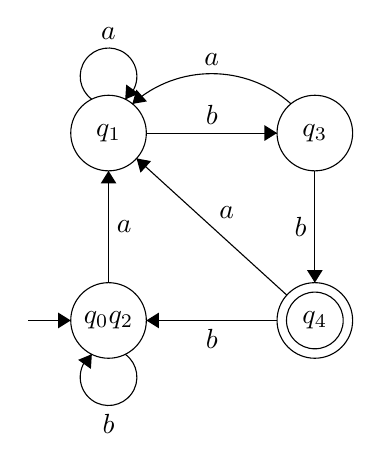
\begin{tikzpicture}[scale=0.2]
            \tikzstyle{every node}+=[inner sep=0pt]
            \draw [black] (5.3,-19.2) circle (2.4);
            \draw (5.3,-19.2) node {$q_0q_2$};
            \draw [black] (5.3,-7.3) circle (2.4);
            \draw (5.3,-7.3) node {$q_1$};
            \draw [black] (18.4,-7.3) circle (2.4);
            \draw (18.4,-7.3) node {$q_3$};
            \draw [black] (18.4,-19.2) circle (2.4);
            \draw (18.4,-19.2) node {$q_4$};
            \draw [black] (18.4,-19.2) circle (1.8);
            \draw [black] (5.3,-16.8) -- (5.3,-9.7);
            \fill [black] (5.3,-9.7) -- (4.8,-10.5) -- (5.8,-10.5);
            \draw (5.8,-13.25) node [right] {$a$};
            \draw [black] (7.7,-7.3) -- (16,-7.3);
            \fill [black] (16,-7.3) -- (15.2,-6.8) -- (15.2,-7.8);
            \draw (11.85,-6.8) node [above] {$b$};
            \draw [black] (18.4,-9.7) -- (18.4,-16.8);
            \fill [black] (18.4,-16.8) -- (18.9,-16) -- (17.9,-16);
            \draw (17.9,-13.25) node [left] {$b$};
            \draw [black] (0.2,-19.2) -- (2.9,-19.2);
            \fill [black] (2.9,-19.2) -- (2.1,-18.7) -- (2.1,-19.7);
            \draw [black] (4.242,-5.156) arc (234:-54:1.8);
            \draw (5.3,-1.4) node [above] {$a$};
            \fill [black] (6.36,-5.16) -- (7.23,-4.8) -- (6.42,-4.22);
            \draw [black] (6.81,-5.448) arc (131.72779:48.27221:7.572);
            \fill [black] (6.81,-5.45) -- (7.74,-5.29) -- (7.07,-4.54);
            \draw (11.85,-3.03) node [above] {$a$};
            \draw [black] (16.62,-17.59) -- (7.08,-8.91);
            \fill [black] (7.08,-8.91) -- (7.33,-9.82) -- (8,-9.08);
            \draw (12.81,-12.76) node [above] {$a$};
            \draw [black] (6.358,-21.344) arc (54:-234:1.8);
            \draw (5.3,-25.1) node [below] {$b$};
            \fill [black] (4.24,-21.34) -- (3.37,-21.7) -- (4.18,-22.28);
            \draw [black] (16,-19.2) -- (7.7,-19.2);
            \fill [black] (7.7,-19.2) -- (8.5,-19.7) -- (8.5,-18.7);
            \draw (11.85,-19.7) node [below] {$b$};
          \end{tikzpicture}
        \end{center}

        \vfill\null
        \columnbreak

        \begin{center}
          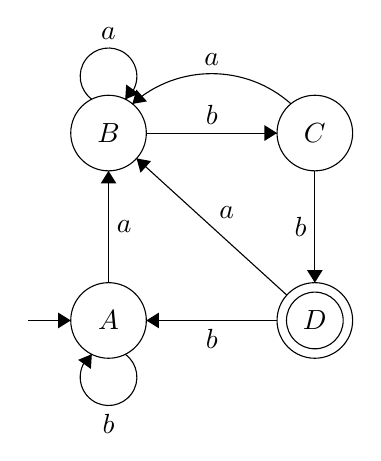
\begin{tikzpicture}[scale=0.2]
            \tikzstyle{every node}+=[inner sep=0pt]
            \draw [black] (5.3,-19.2) circle (2.4);
            \draw (5.3,-19.2) node {$A$};
            \draw [black] (5.3,-7.3) circle (2.4);
            \draw (5.3,-7.3) node {$B$};
            \draw [black] (18.4,-7.3) circle (2.4);
            \draw (18.4,-7.3) node {$C$};
            \draw [black] (18.4,-19.2) circle (2.4);
            \draw (18.4,-19.2) node {$D$};
            \draw [black] (18.4,-19.2) circle (1.8);
            \draw [black] (5.3,-16.8) -- (5.3,-9.7);
            \fill [black] (5.3,-9.7) -- (4.8,-10.5) -- (5.8,-10.5);
            \draw (5.8,-13.25) node [right] {$a$};
            \draw [black] (7.7,-7.3) -- (16,-7.3);
            \fill [black] (16,-7.3) -- (15.2,-6.8) -- (15.2,-7.8);
            \draw (11.85,-6.8) node [above] {$b$};
            \draw [black] (18.4,-9.7) -- (18.4,-16.8);
            \fill [black] (18.4,-16.8) -- (18.9,-16) -- (17.9,-16);
            \draw (17.9,-13.25) node [left] {$b$};
            \draw [black] (0.2,-19.2) -- (2.9,-19.2);
            \fill [black] (2.9,-19.2) -- (2.1,-18.7) -- (2.1,-19.7);
            \draw [black] (4.242,-5.156) arc (234:-54:1.8);
            \draw (5.3,-1.4) node [above] {$a$};
            \fill [black] (6.36,-5.16) -- (7.23,-4.8) -- (6.42,-4.22);
            \draw [black] (6.81,-5.448) arc (131.72779:48.27221:7.572);
            \fill [black] (6.81,-5.45) -- (7.74,-5.29) -- (7.07,-4.54);
            \draw (11.85,-3.03) node [above] {$a$};
            \draw [black] (16.62,-17.59) -- (7.08,-8.91);
            \fill [black] (7.08,-8.91) -- (7.33,-9.82) -- (8,-9.08);
            \draw (12.81,-12.76) node [above] {$a$};
            \draw [black] (6.358,-21.344) arc (54:-234:1.8);
            \draw (5.3,-25.1) node [below] {$b$};
            \fill [black] (4.24,-21.34) -- (3.37,-21.7) -- (4.18,-22.28);
            \draw [black] (16,-19.2) -- (7.7,-19.2);
            \fill [black] (7.7,-19.2) -- (8.5,-19.7) -- (8.5,-18.7);
            \draw (11.85,-19.7) node [below] {$b$};
          \end{tikzpicture}
        \end{center}
      \end{multicols}
  \end{itemize}
\end{examplebreak}


\subsection{Myhill Nerode Theorem}

\begin{multicols}{2}
\setlength{\columnsep}{1.5cm}
\setlength{\columnseprule}{0.2pt}

\begin{enumerate}
  \item Create the pairs of all the states involved in the given DFA.
  \item Mark all the pairs $(Q_a, Q_b)$ such a that $Q_a$ is Final state and $Q_b$ is Non-Final State or vice versa.
  \item If there is any unmarked pair $(Q_a, Q_b)$ such a that $\delta(Q_a, x)$ and $\delta(Q_b, x)$ is marked, then mark $(Q_a, Q_b)$. Here $x$ is a input symbol. Repeat this step until no more marking can be made.
  \item Combine all the unmarked pairs and make them a single state in the minimized DFA.
\end{enumerate}

\vfill\null
\columnbreak

This way is quite cumbersome and prone to errors. Check the following links for examples:

\begin{figure}[H]
  \centering
  \includegraphics[width=.2\textwidth]{img/minizimation-1.png}
  \caption{\href{https://bit.ly/3xVGyMD}{https://bit.ly/3xVGyMD}}
\end{figure}

\begin{figure}[H]
  \centering
  \includegraphics[width=.2\textwidth]{img/minizimation-2.png}
  \caption{\href{https://bit.ly/3Oxj9Xw}{https://bit.ly/3Oxj9Xw}}
\end{figure}

\end{multicols}
